\documentclass[12pt, a4paper, onside]{article}
\usepackage[affil-it]{authblk} % author institution
\usepackage{graphicx}
\usepackage{pythonhighlight}

\title{\textbf{Internet of Things: Technologies and Applications -- Lab 6}}
\author{Tran Phong Binh\thanks{Department of Computer Science, Student ID: 110062421}, Hao-Shan Yuan\thanks{Institute of Information Systems and Applications, Student ID: 110065507}}
\affil{National Tsing Hua University}
\date{\today}

\begin{document}

\maketitle

\section{Introduction}
We aim to build the following system:
\begin{itemize}
  \item Two Raspberry Pis are connected by Bluetooth, being either server (master) or client (slave).
  \item The server listens to user's speech commands, which are confined to five options: `activate white socket', `deactivate white socket', `activate yellow socket', `deactivate yellow socket', and `retrieve information'.
  \item The server sends the speech command to the client for processing.
  \item The client activates/deactivates white/yellow socket -- turns on/off respective electronic devices, or retrieves AC information from PZEM004T according to the given request.
  \item The client transmits a task failure/success message or the read AC information to the server.
  \item The server plays the received packet by audio for the user.
\end{itemize}

\section{Setup}
Our experiment's setup is demonstrated by the figures below:
\begin{figure}[h]
  \centering
  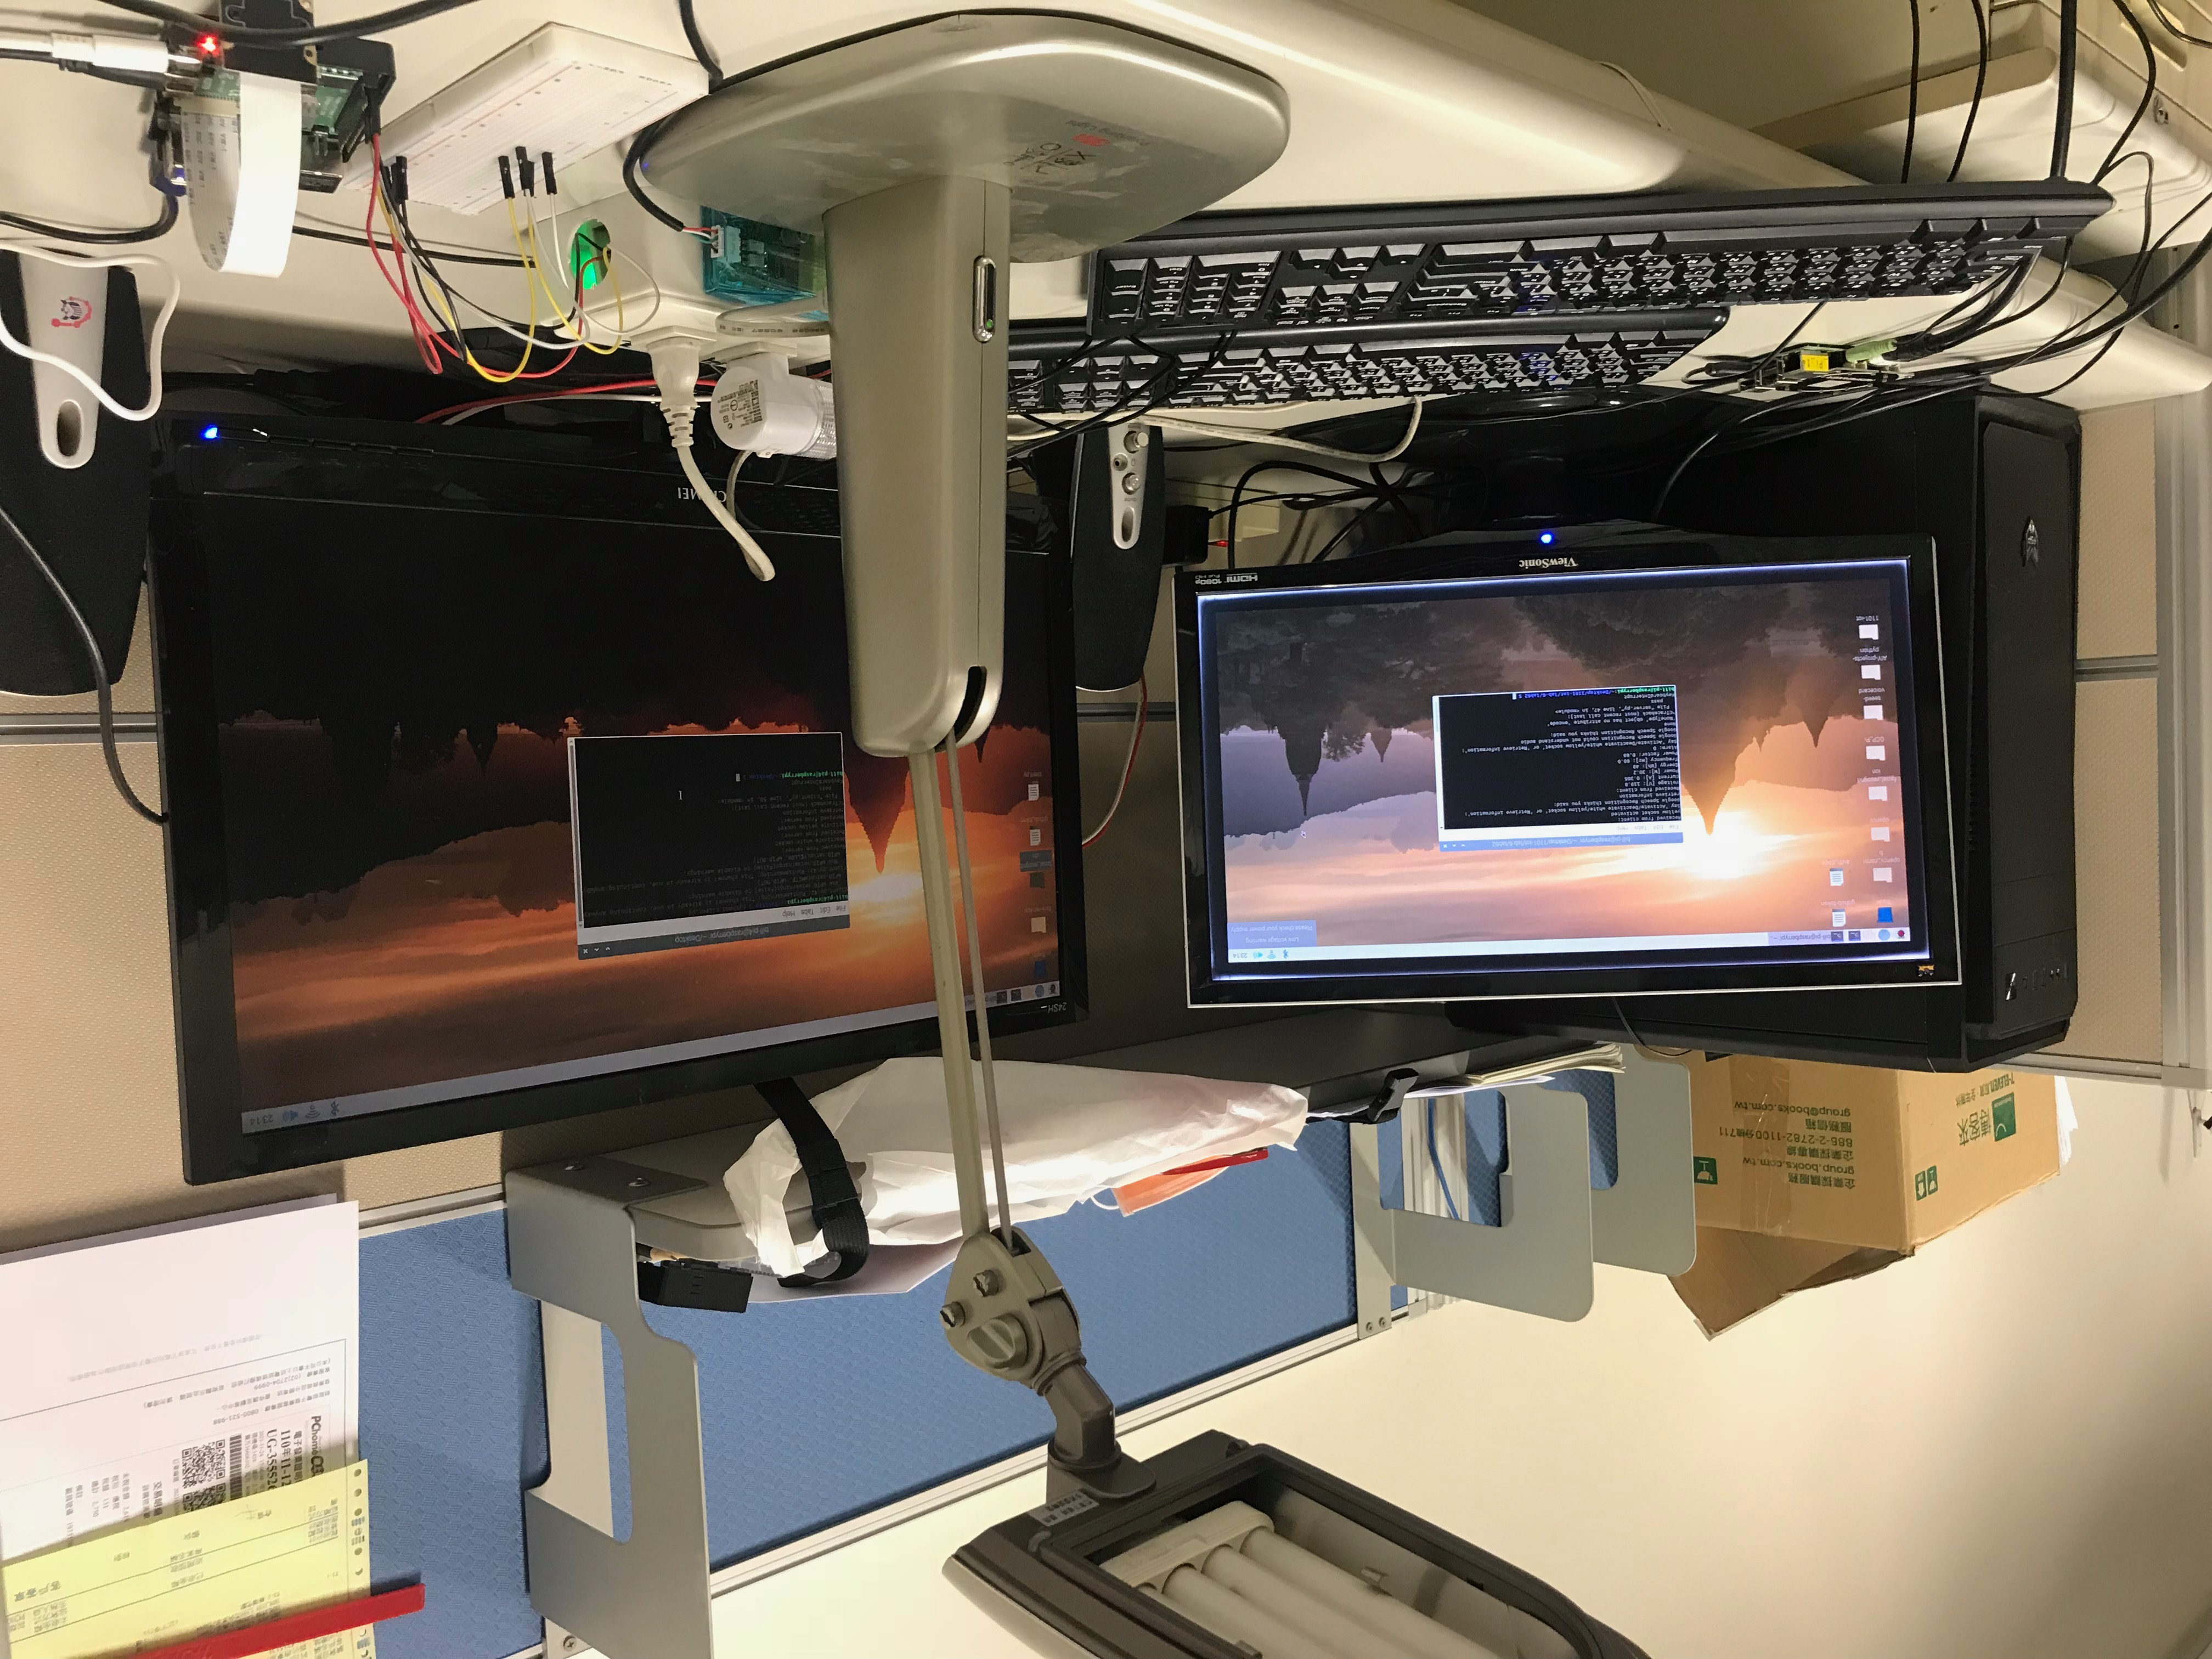
\includegraphics[angle=180, origin=c, width=0.6\textwidth]{img/overall_setup}
  \caption{Overall setup}
\end{figure}
\begin{figure}[h]
  \centering
  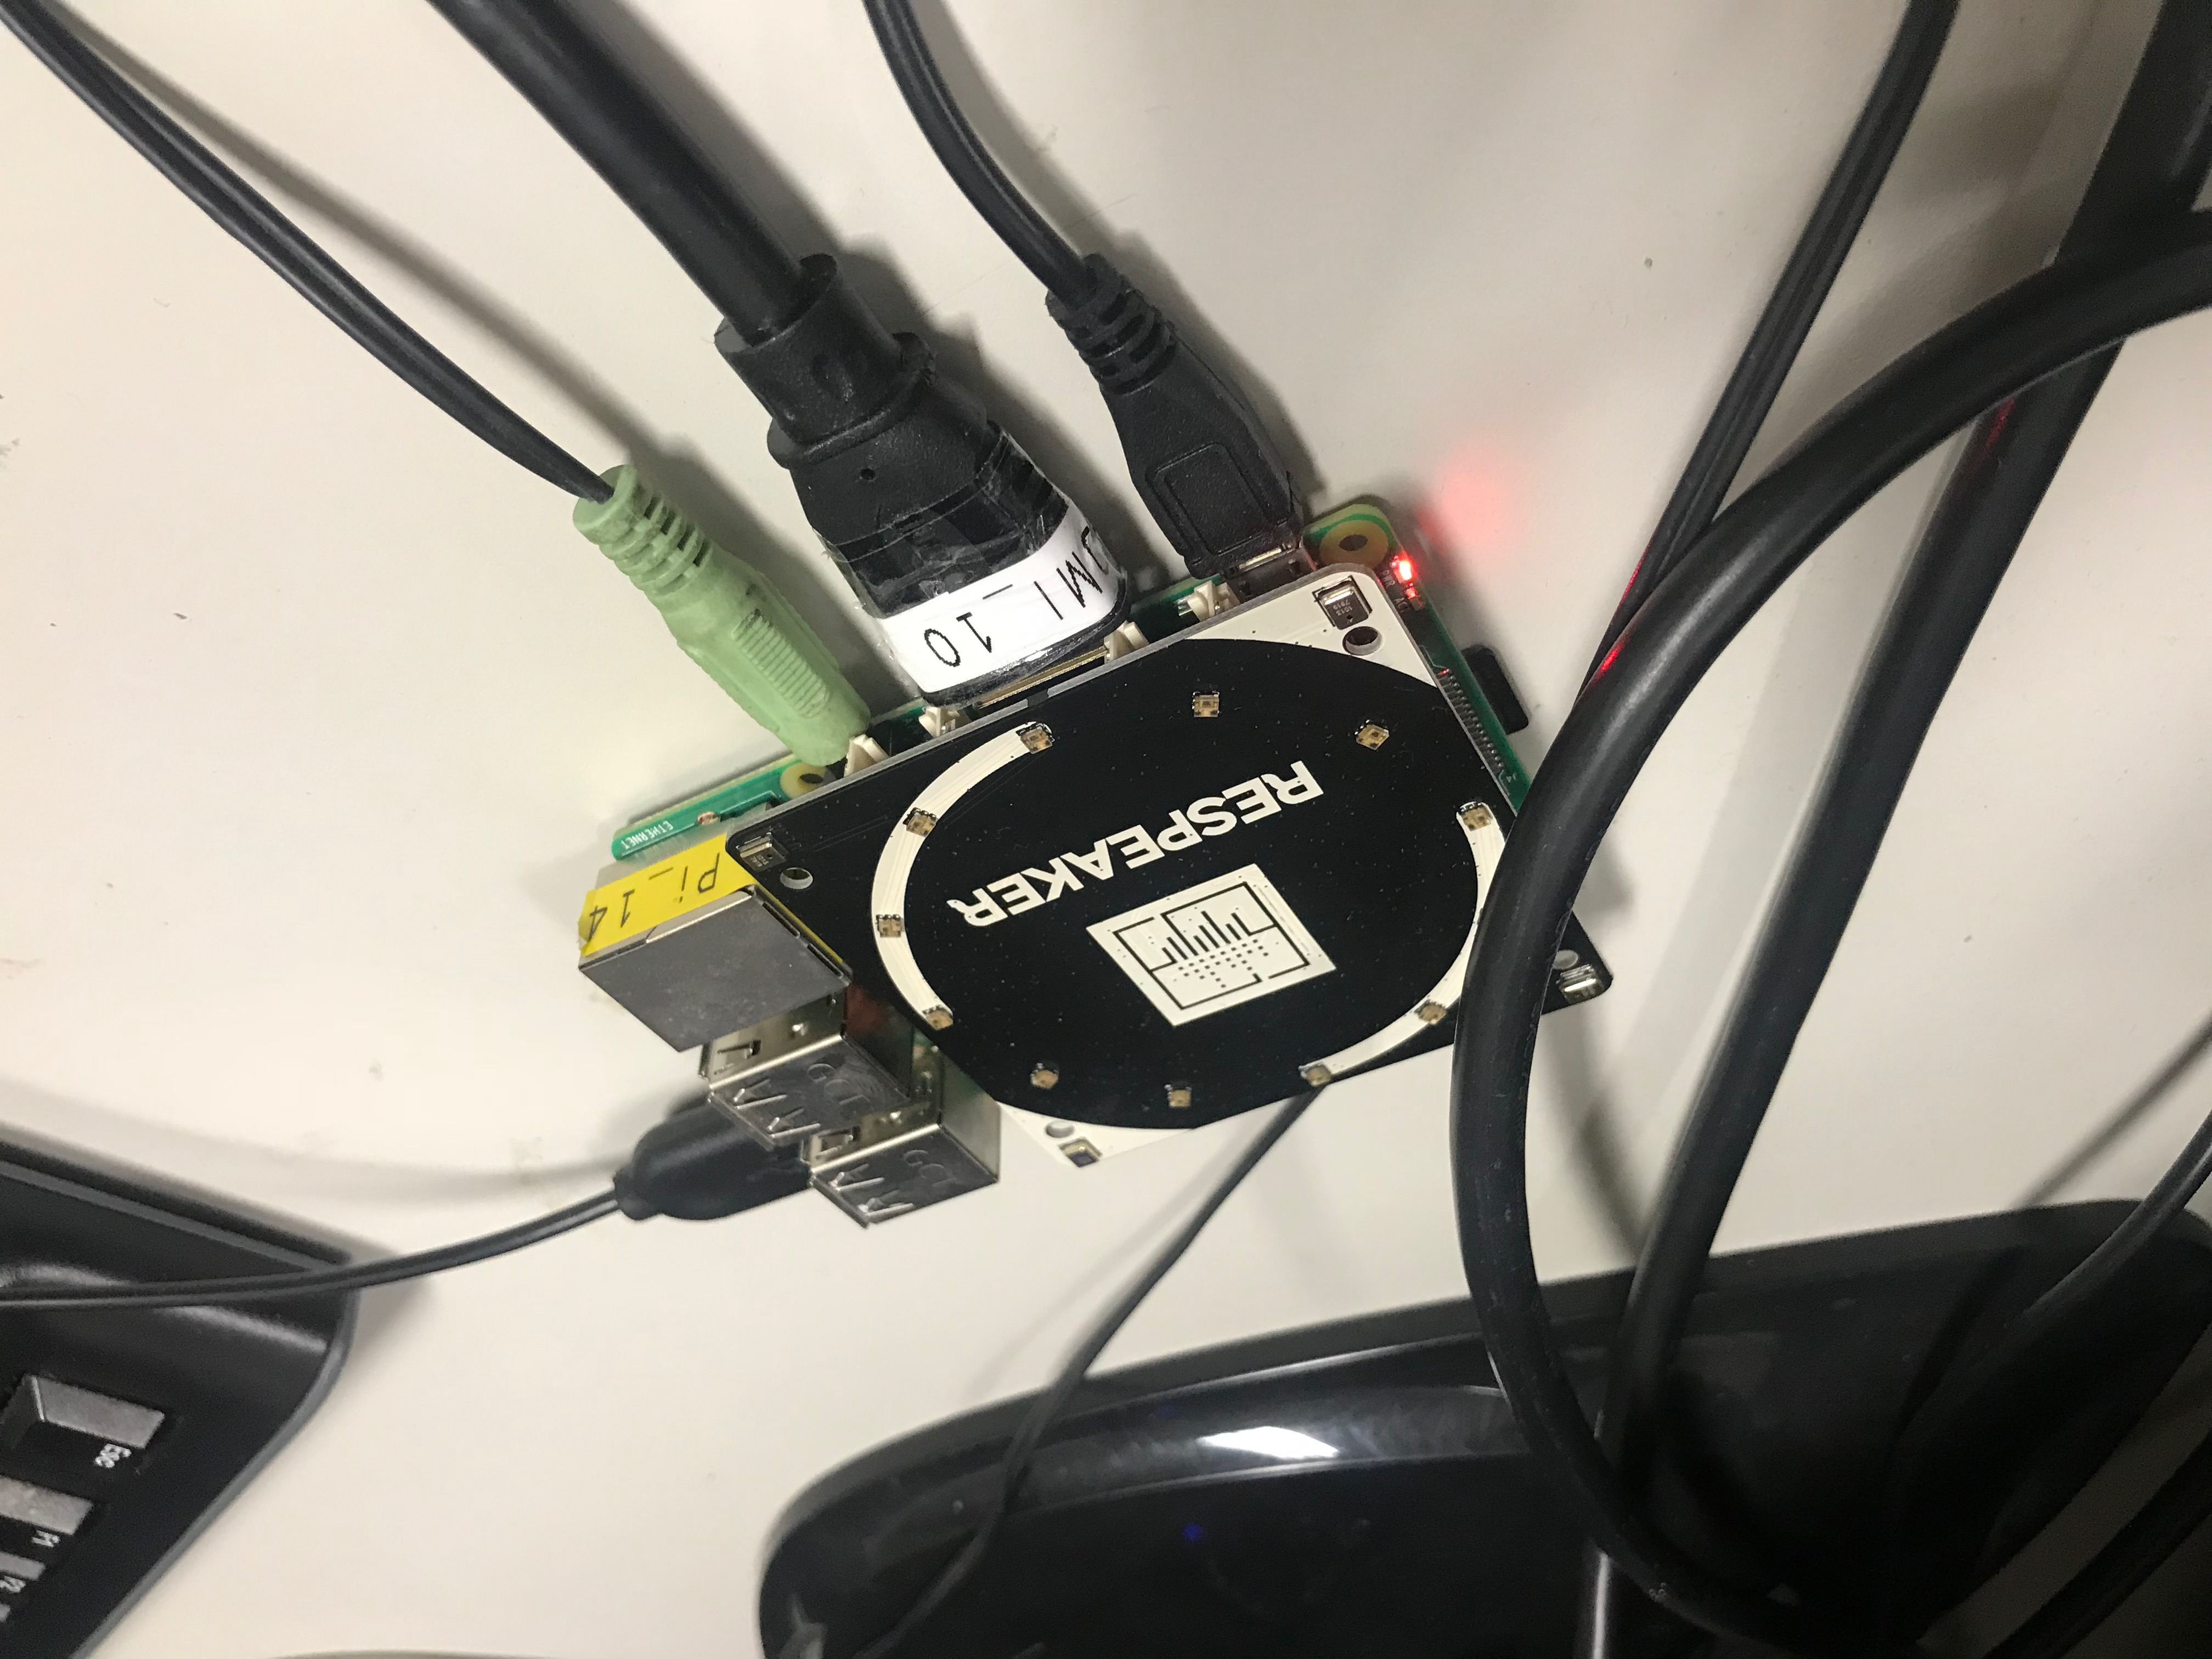
\includegraphics[angle=180, origin=c, width=0.6\textwidth]{img/server_setup}
  \caption{Server setup: a speech module installed directly on GPIO pins and a pair of speakers plugged in by the green jacket}
\end{figure}
\begin{figure}[h]
  \centering
  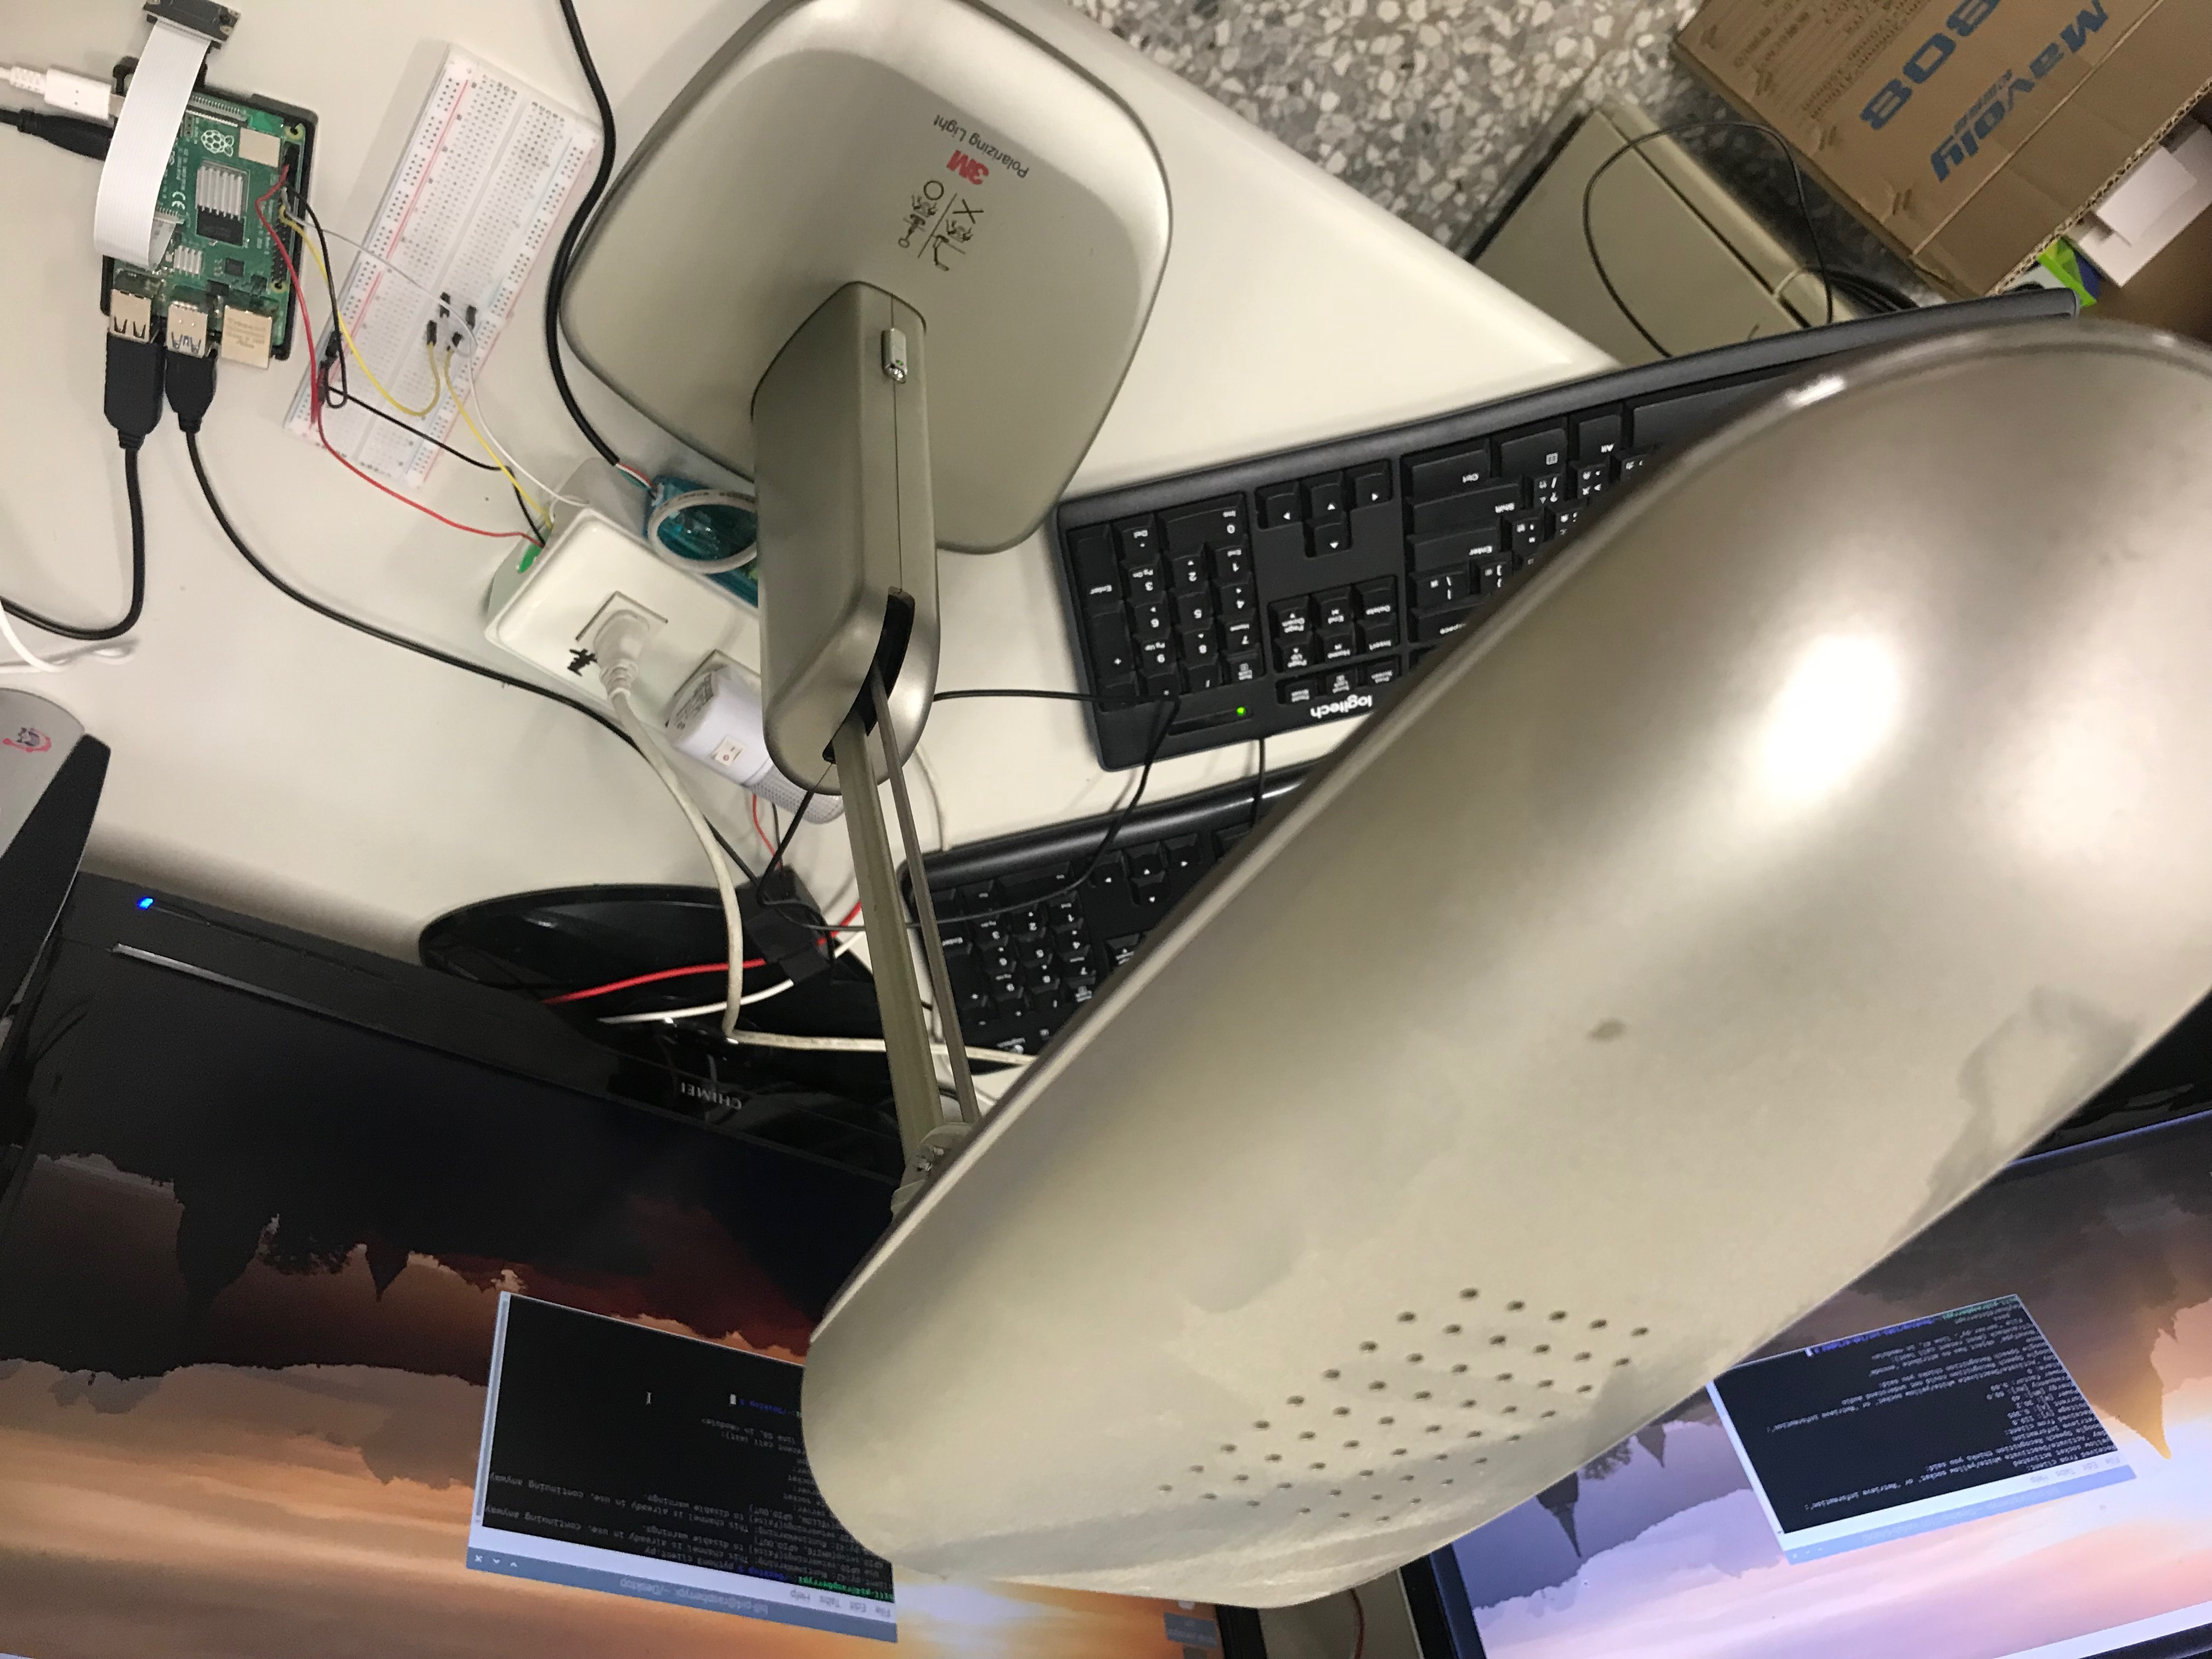
\includegraphics[angle=180, origin=c, width=0.6\textwidth]{img/client_setup}
  \caption{Client setup}
\end{figure}
\begin{figure}[h]
  \centering
  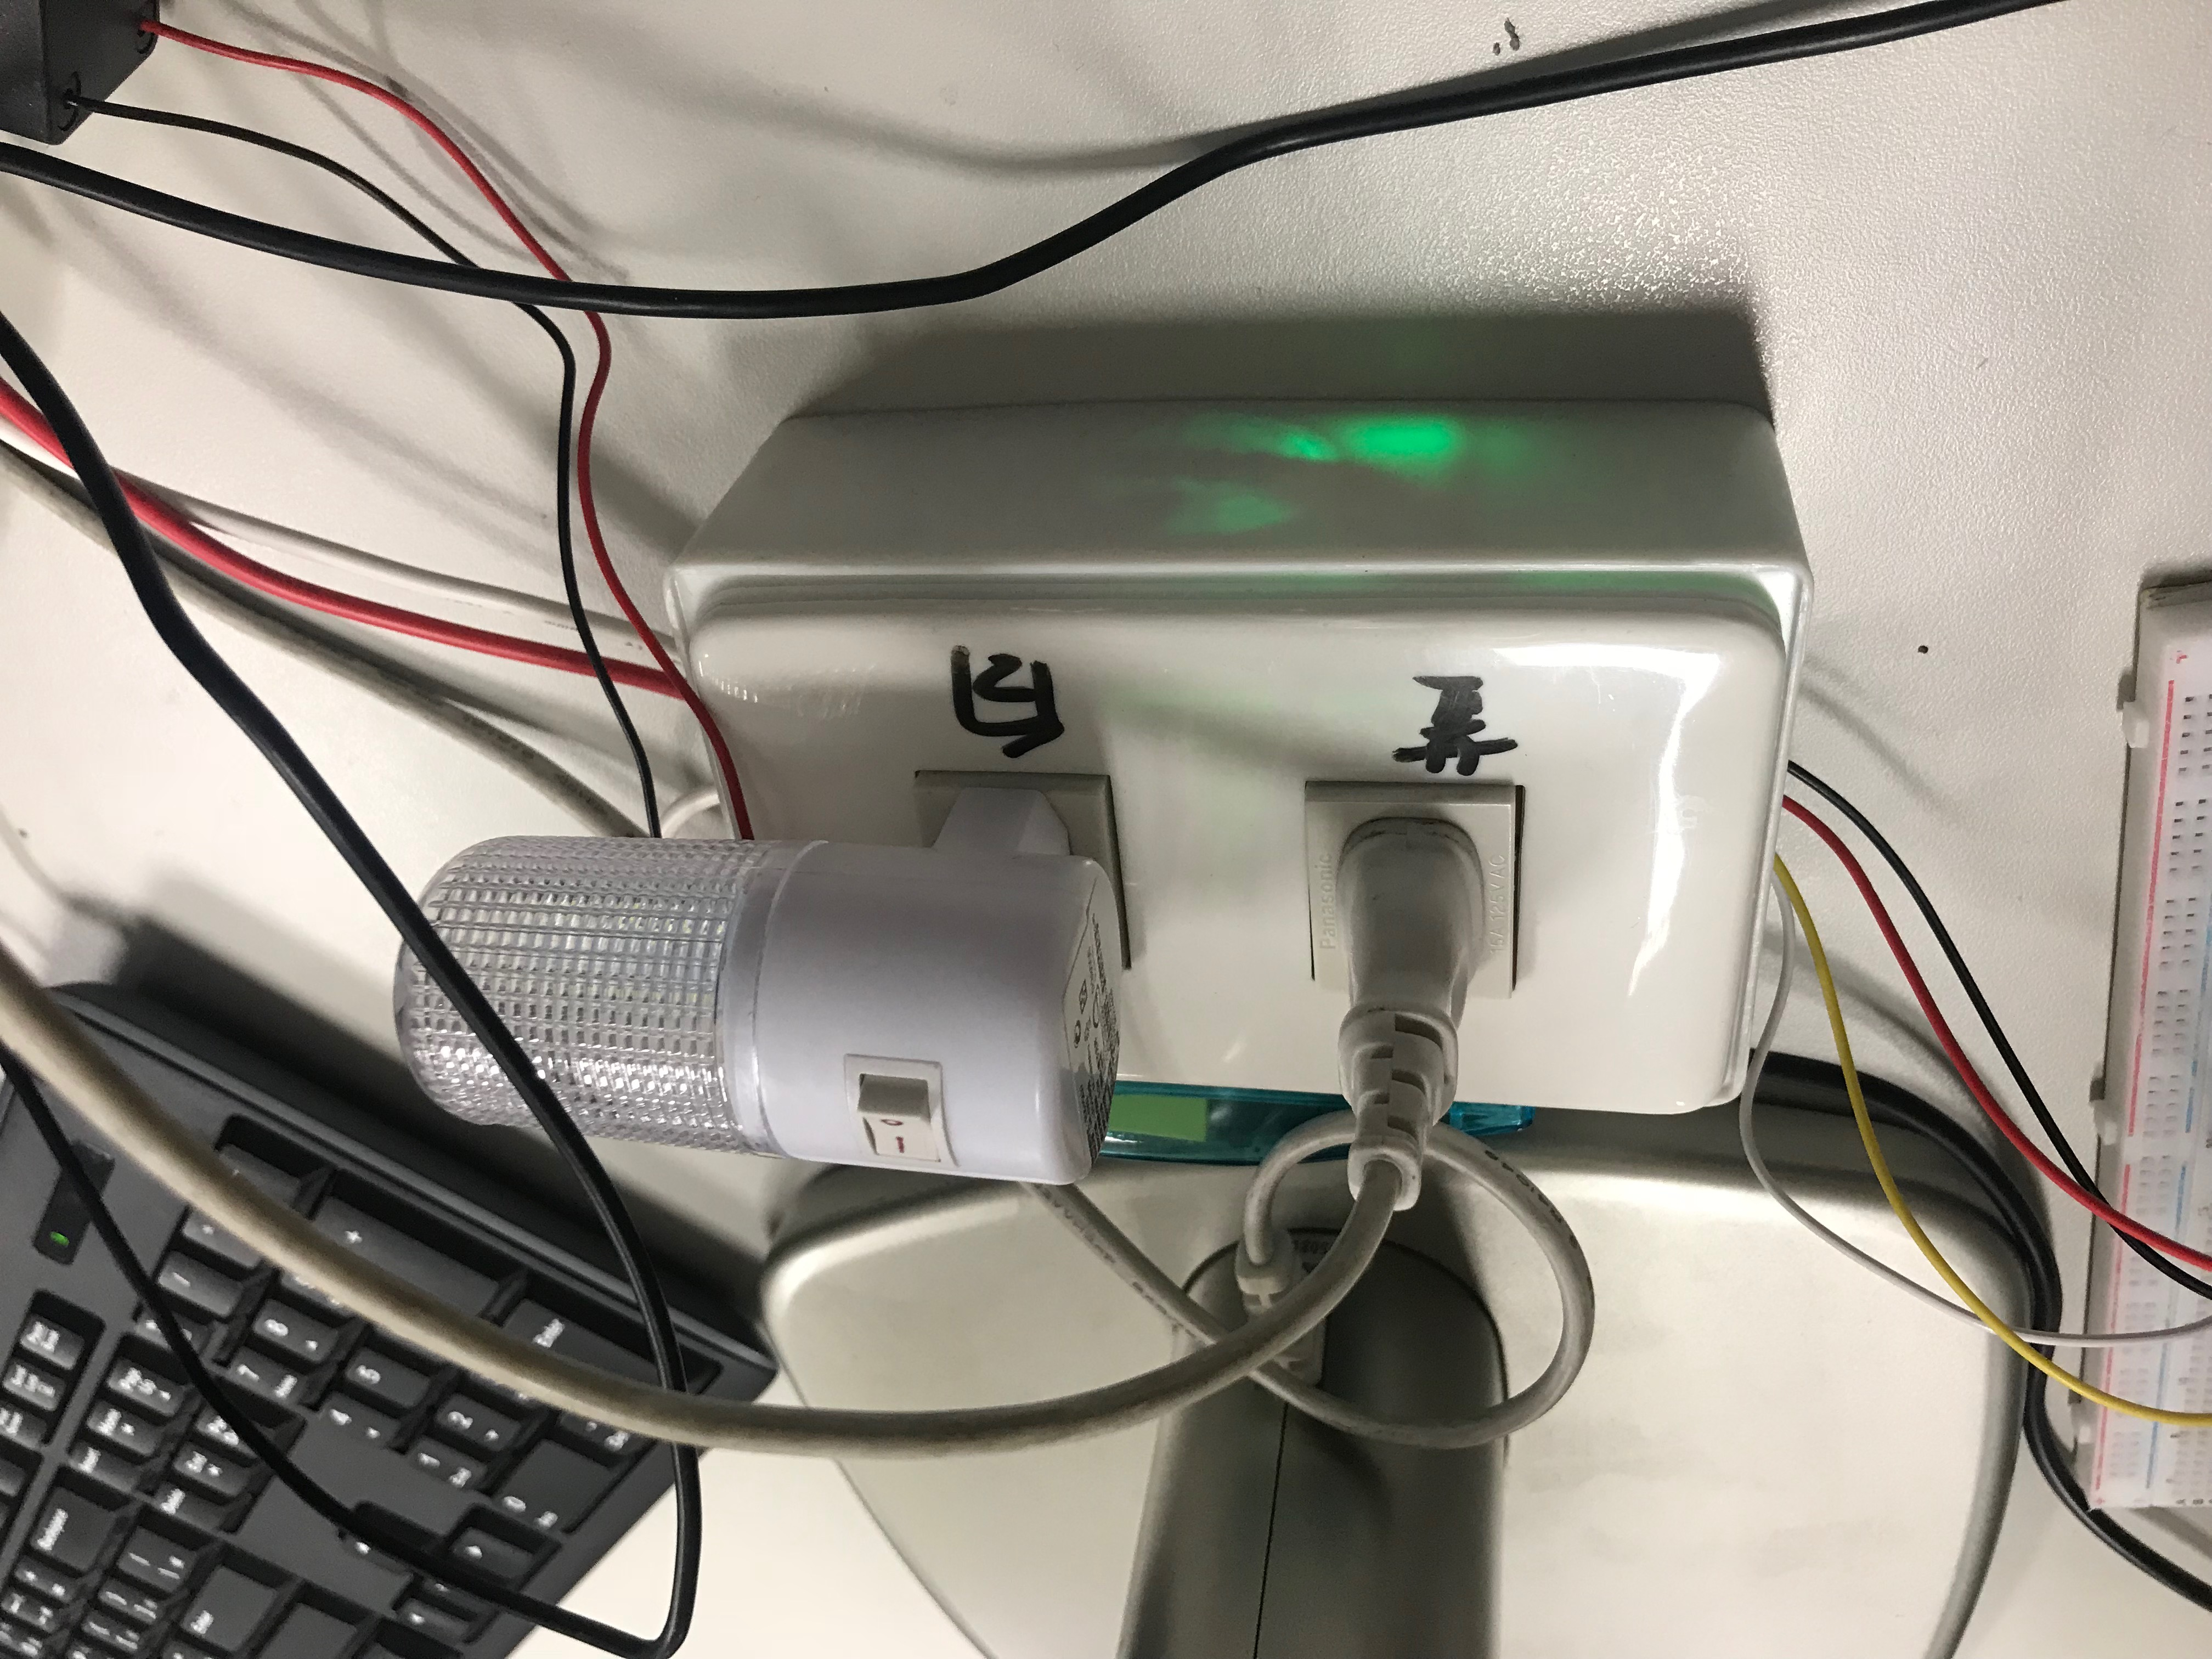
\includegraphics[angle=180, origin=c, width=0.6\textwidth]{img/client_sockets}
  \caption{Client sockets: yellow to the left corresponds to the table lamp, with white to the right powering the LED light}
\end{figure}
\begin{figure}[h]
  \centering
  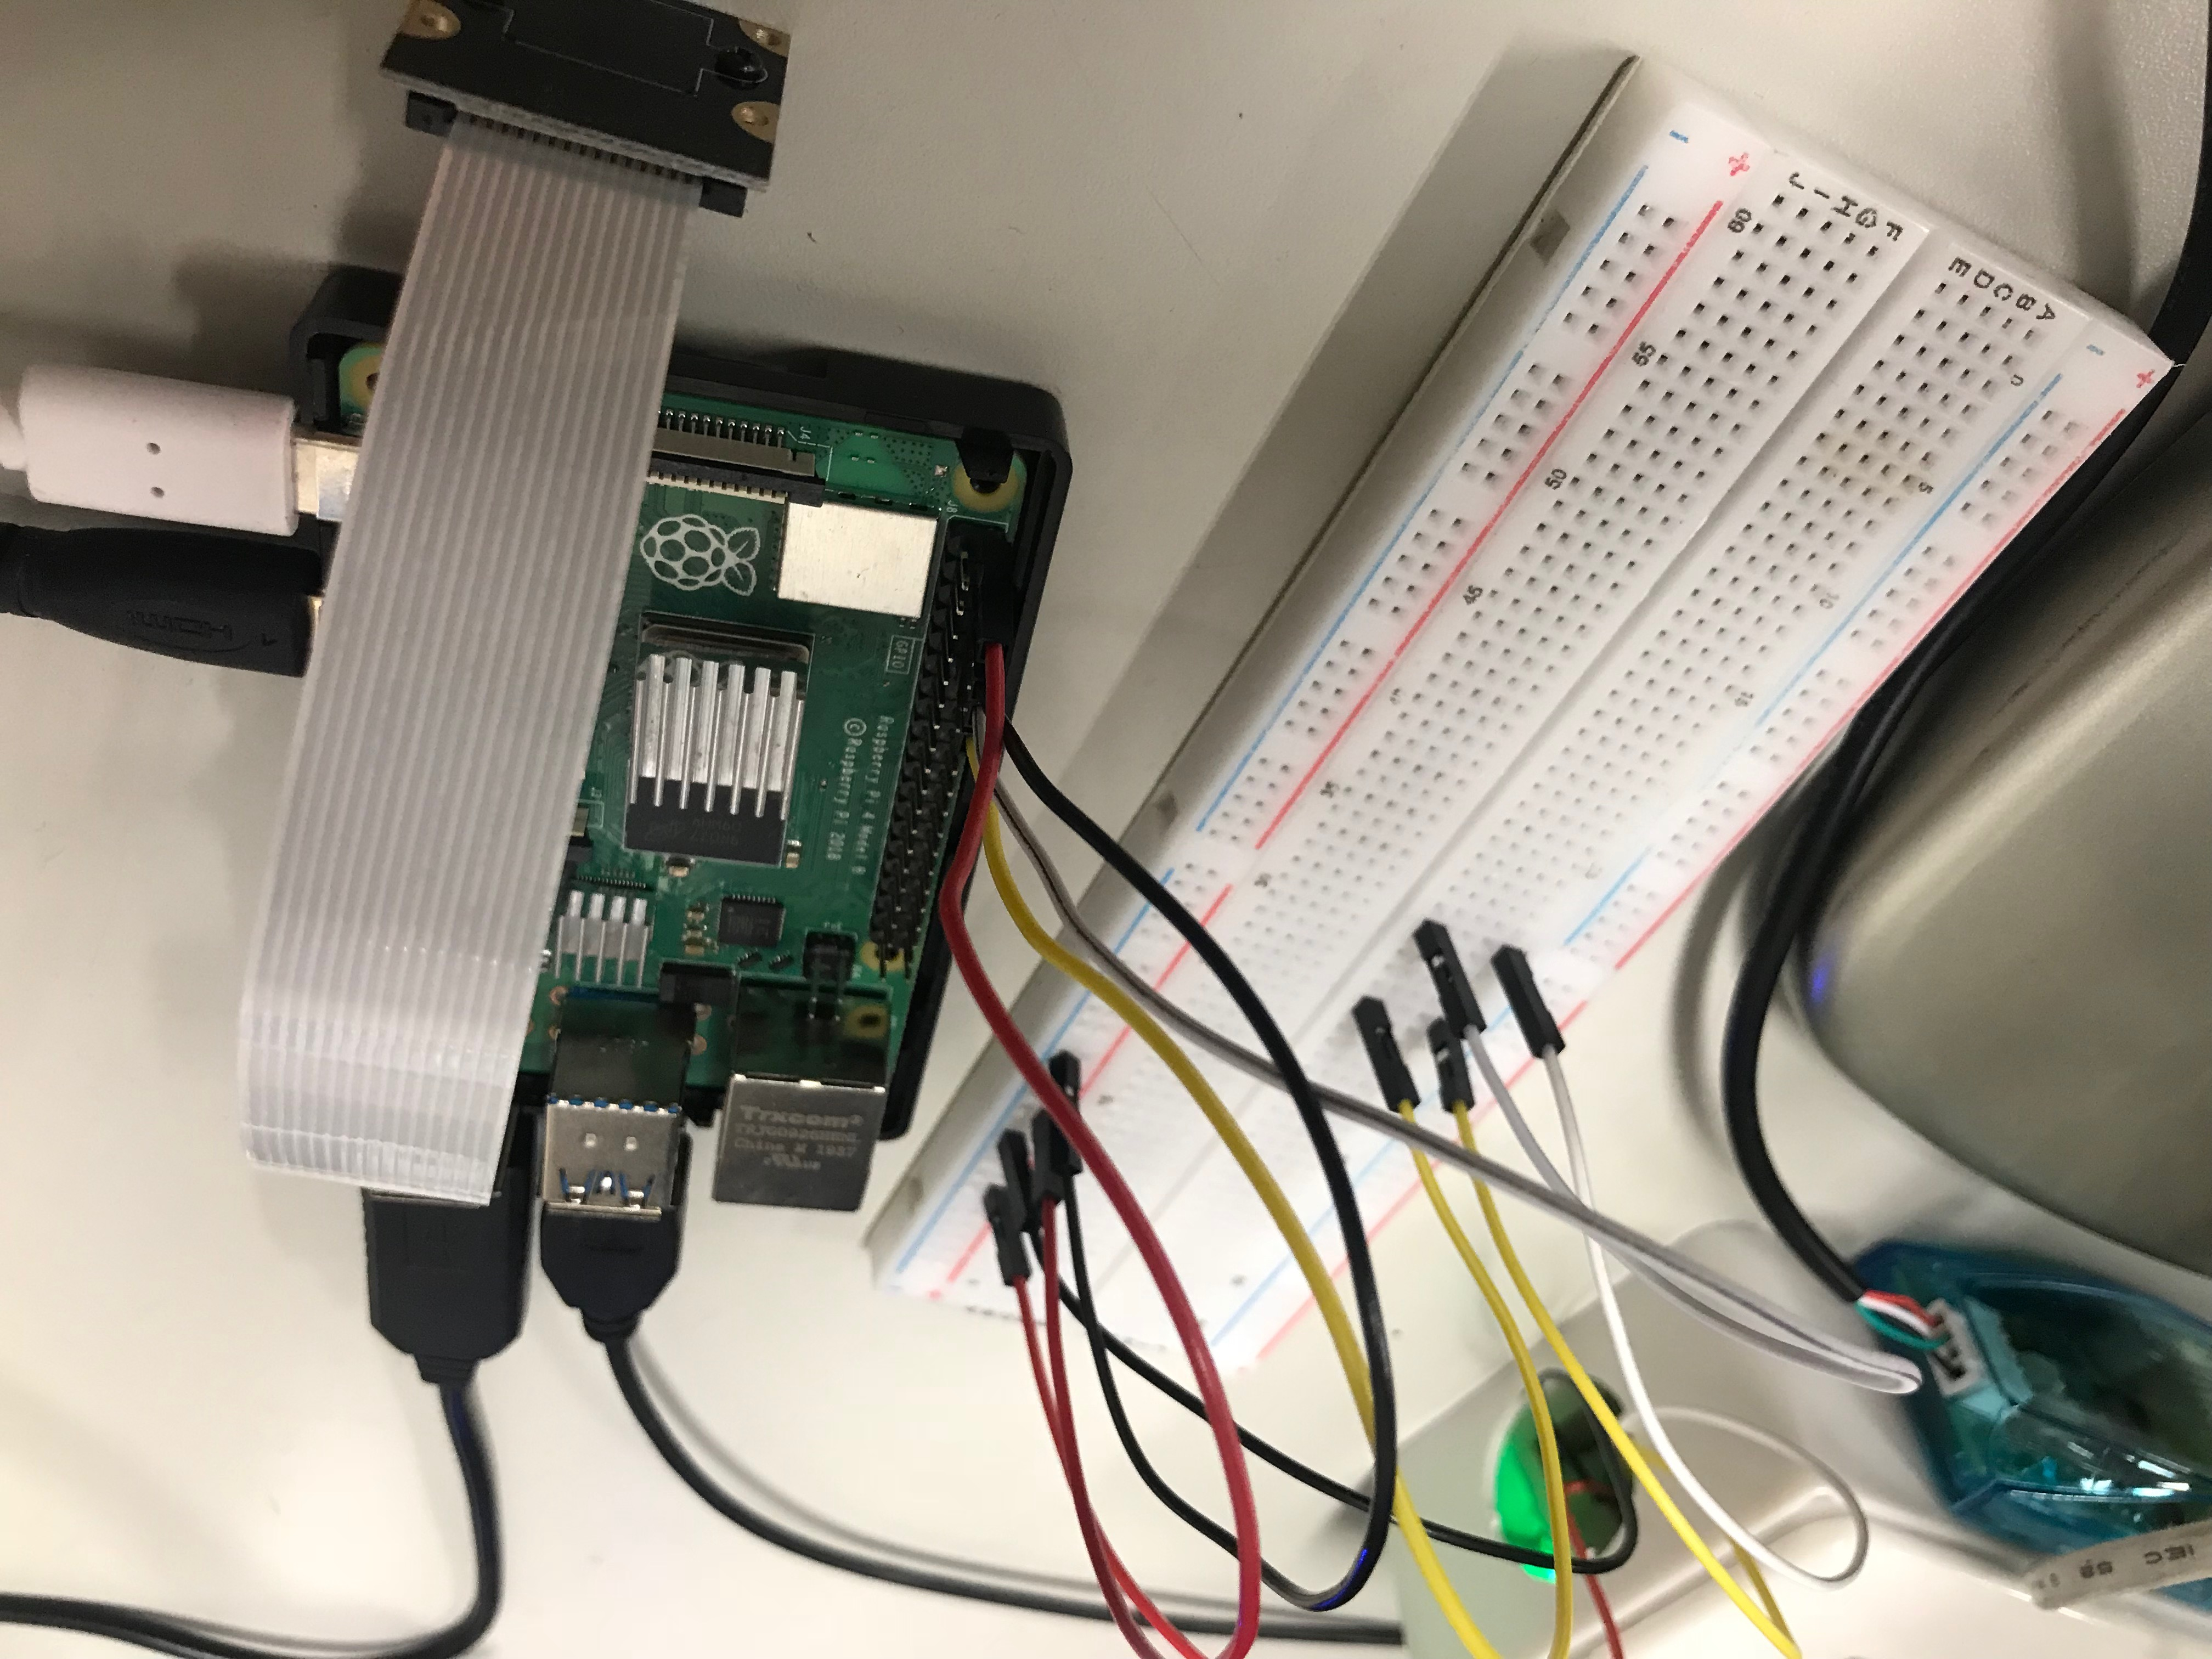
\includegraphics[angle=180, origin=c, width=0.6\textwidth]{img/client_circuit}
  \caption{Client circuit: white socket is directed to GPIO 14, with yellow to GPIO 15}
\end{figure}

\clearpage

\section{Implementation}
We begin by pairing our Raspberry Pis. Since a Bluetooth master can serve 7 active slaves simultaneously, we must identify our slave to the master by sending a message (here as `initiate connection') from our client end. Once the two devices are bonded, the server starts listening to user's speech command using Speech-to-Text service provided by Google. The server then sends its interpretation to the server. If the command conforms with the format stated in the introduction section above, the client executes the job (we chose not to explain the details here because they have already been described in previous labs), transmitting a success message or the read AC information back to the server. Otherwise, the client yields the message `the given command does not exist', indicating a failed operation with the server. The server then uses Google Speech's Text-to-Speech to play the packet returned via its speakers. After the audio finishes playing, the server awaits the next command from the user, and the whole process is repeated. Our implementation is illustrated in the two subsections below.

\subsection{Server}
\begin{python}
import speech_recognition
from bluedot.btcomm import BluetoothServer
import tempfile
from gtts import gTTS
from pygame import mixer
import time

def get_message():
    r = speech_recognition.Recognizer()
    with speech_recognition.Microphone() as source:
      r.adjust_for_ambient_noise(source, duration=1)
      print("Say 'Activate/Deactivate white/yellow socket' or 'Retrieve information':")
      audio = r.listen(source)
    try:
      return r.recognize_google(audio, language="en-US")
    except speech_recognition.UnknownValueError:
      print("Google Speech Recognition could not understand audio")
    except sr.RequestError as e:
      print("No response from Google Speech Recognition serve: {0}".format(e))

def play(sentence, lang, loops_count):
  with tempfile.NamedTemporaryFile(delete=True) as file:
    tts = gTTS(text=sentence, lang=lang)
    tts.save('{}.mp3'.format(file.name))
    mixer.init()
    mixer.music.load('{}.mp3'.format(file.name))
    mixer.music.play(loops_count)

def receive_client_message(client_msg):
  print("Received from client:")
  print(client_msg)
  try:
    play(client_msg, 'en', 1)
    if len(client_msg) > 50:
      time.sleep(25)
    else:
      time.sleep(2)
    msg = get_message()
    print("Google Speech Recognition thinks you said:")
    print(msg)
    s.send(msg)
  except Exception as e:
    print(e)

s = BluetoothServer(receive_client_message)
while True: # for bluetooth server to listen
  pass
\end{python}

\subsection{Client}
\begin{python}
from bluedot.btcomm import BluetoothClient
import RPi.GPIO as GPIO
import serial
import modbus_tk.defines as cst
from modbus_tk import modbus_rtu

WHITE = 14
YELLOW = 15

def get_ac_info():
  data = master.execute(1, cst.READ_INPUT_REGISTERS, 0, 10)
  voltage     =   data[0]                     / 10.0   # [V]
  current     = ( data[1] + (data[2] << 16) ) / 1000.0 # [A]
  power       = ( data[3] + (data[4] << 16) ) / 10.0   # [W]
  energy      =   data[5] + (data[6] << 16)            # [Wh]
  frequency   =   data[7]                     / 10.0   # [Hz]
  powerFactor =   data[8]                     / 100.0
  alarm       =   data[9]                              # 0 means no alarm
  return 'Voltage [V]: ' + str(voltage) + '\n' + 'Current [A]: ' + str(current) + '\n' + 'Power [W]: ' + str(power) + '\n' + 'Energy [Wh]: ' + str(energy) + '\n' + 'Frequency [Hz]: ' + str(frequency) + '\n' + 'Power factor: ' + str(powerFactor) + '\n' + 'Alarm: ' + str(alarm)

def receive_server_msg(msg):
  print("Received from server:")
  print(msg)
  if msg == "activate white socket":
    GPIO.output(WHITE, GPIO.HIGH)
    c.send("white socket activated")
  elif msg == "deactivate white socket":
    GPIO.output(WHITE, GPIO.LOW)
    c.send("white socket deactivated")
  elif msg == "activate yellow socket":
    GPIO.output(YELLOW, GPIO.HIGH)
    c.send("yellow socket activated")
  elif msg == "deactivate yellow socket":
    GPIO.output(YELLOW, GPIO.LOW)
    c.send("yellow socket deactivated")
  elif msg == "retrieve information":
    c.send(get_ac_info())
  else:
    c.send("the given command does not exist")

GPIO.setmode(GPIO.BCM)
GPIO.setup(WHITE, GPIO.OUT)
GPIO.setup(YELLOW, GPIO.OUT)
sensor = serial.Serial(
#  port='/dev/PZEM_sensor',
  port='/dev/ttyUSB0',
  baudrate=9600,
  bytesize=8,
  parity='N',
  stopbits=1,
  xonxoff=0)
master = modbus_rtu.RtuMaster(sensor)
master.set_timeout(2.0)
master.set_verbose(True)
c = BluetoothClient("phogbinh", receive_server_msg)
c.send("initiate connection")
while True:
  pass
\end{python}

\section{Result}
The result of our experiment is shown here: \texttt{https://youtu.be/guJDFmyFZh0}.

\end{document}
